\section{Is the Cast Operator used?}
\label{sec:casts:stats}







To achieve our goal, several elements are needed.

\textbf{Source Code Analysis.}
We have implemented our study using the \ql{} query language:
``a declarative, object-oriented logic programming language for querying complex, potentially recursive data structures encoded in a relational data model''~\citep{avgustinovQLObjectorientedQueries2016}.
\ql{} allows us to analyze programs at the source code level by abstracting the code sources into a Datalog model.
Besides providing structural data for programs, \ie{}, ASTs,
\ql{} has the ability to query static types and perform data-flow analysis.
To run our \ql{} queries, we have used the service provided by Semmle.\footnote{\url{https://lgtm.com/}} 

\textbf{Projects.} 
As a code base representative of the ``real world'',
we have chosen open-source projects hosted in 
\github{},
the world-most popular source code management repository.
% , \ie{},
% \github{},
%\footnote{\url{https://github.com/}},
% \gitlab{},
%\footnote{\url{https://gitlab.com/}},
% \bitbucket{},
%\footnote{\url{https://bitbucket.org/}}.
So far, we have analyzed \nproject{} \java{} projects in \lgtm{}.
We plan to scale up our analysis to the whole \lgtm{} project database.

\textbf{Usage Pattern Detection.}
After all cast instances are found, we analyze this information to discover usage patterns.
\ql{} allows us to automatically categorize cast use cases into patterns.
This methodology is described in section~\ref{sec:casts:methodology}.

Our list of patterns is not exhaustive.
Due to the nature of the cast operator, some casts were uncategorized as they would need a whole program analysis, \eg{}, including libraries in the analysis.









To answer \ref{casts:rq1} (\emph{\crqA}) we want to know how many cast instances are used in a given project.
To this end, we gather the following statistics using \ql{}.
We show them here to give an estimation of the size of the code base being analized.
% DONE: Why only 24 project? Should say this is preliminary?
As mentioned above, these results are preliminary.
We plan to scale up our analysis to the whole \lgtm{} project database.

\begin{center}
\begin{tabular}{lr}
	Description & Value\\
	\hline
	Number of Projects & \nproject \\
	Number of LOC & \nloc{} \\
	Number of Methods & \nmethod \\
	Number of Methods \emph{w/}Cast & \nmethodwithcast \\
    Number of Expressions & \nexpr \\
	\hline
    Number of Cast Expressions & \nCastExpr \\
    Number of Cast Methods & \nCastMethod \\
    Number of \code{equals} Methods & \nEqualsMethod \\
    Number of \code{instanceof} Expressions & \nInstanceOf \\
    Number of type switch & \nTypeSwitch \\
\end{tabular}
\end{center}

The \emph{Number of Methods} and \emph{Number of Methods w/Cast} values includes only methods with a body, \ie{}, not abstract, nor native.
The \emph{Number of Exprs} value show how many expressions there are in the ASTs of all source code analyzed.
Finally, the \emph{Number of Casts} value indicates how many cast expressions (subtype of \code{Expr} as defined by \ql{}) were found.

% DONE: This is why, no?: Better explained
For our study, we are interested in both upcasts and downcasts.
Thus, we \emph{exclude} primitive conversions in our study
(\S$5.1.2$, \S$5.1.3$, \S$5.1.4$, and \S$5.1.13$ from the \java{} Language Specification%
\footnote{\url{https://docs.oracle.com/javase/specs/jls/se7/html/jls-5.html}}
).
The \emph{Number of Casts} value shown above include only reference conversions.
Primitive conversions are always safe (in terms of throwing \code{ClassCastException}.
A primitive conversion happens when both the type of the expression to be casted to and
the type to cast to are primitive types.
Note that with this definition, we include in our study \emph{boxed} types.
Since boxed types are reference types (and therefore not necessarily safe)
we want to include them in our analysis.

We want to know how many cast instances there are across projects.
Thus, we have computed the ratio between methods containing
at least a cast over total number of methods --- with implementation --- in a given project.
The following chart shows this ratio for all analyzed projects:

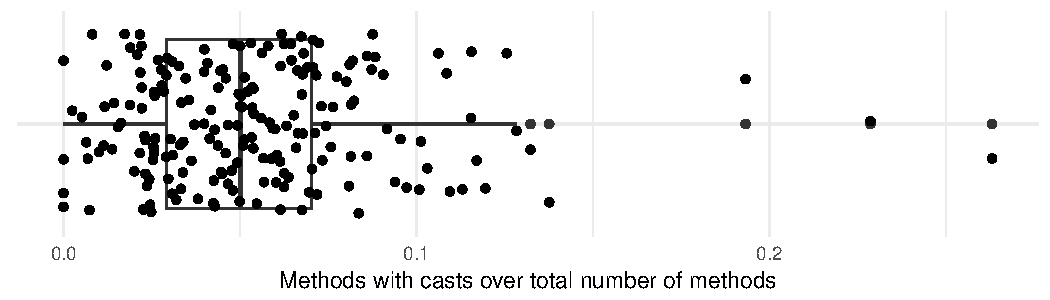
\includegraphics[width=0.9\columnwidth]{analysis/stats-methodwcastXproject.pdf}

All projects have less than 10\% of methods with at least a cast.
Overall, around a \castpercentage{}\% of methods contain at least one cast operation. 
This means there is a low density of casts.
Given the fact that generics were introduced \java{} 5, this can explain this low density.

Nevertheless, casts are still used.
We want to understand why there are casts instances (\ref{casts:rq2}) and how often the use cases that leads to casts are used (\ref{casts:rq3}).
The following sections give an answer to these questions.

% DONE: cut
% The query to gather this statistics is available online.\footnote{\url{https://gitlab.com/acuarica/java-cast-queries/blob/master/ql/stats.ql}}
% The \lang{R} script to further analyze the query results is available online as well.\footnote{\url{https://gitlab.com/acuarica/java-cast-queries/blob/master/analysis/stats.r}}
